\documentclass{article}
\usepackage[utf8]{inputenc}

\title{Advanced Programming Labwork 4}
\author{Tom HERBRETEAU }
\date{October 2018}

\usepackage{natbib}
\usepackage{graphicx}
\usepackage{pgfplots}
\pgfplotsset{compat=newest}

\begin{document}

\maketitle
Every performance measures are done on ICT4 with eiffel.jpg, without counting the image saving.
\section{Introduction}
We run the lab 3 with a 2D kernel.
\section{Result}
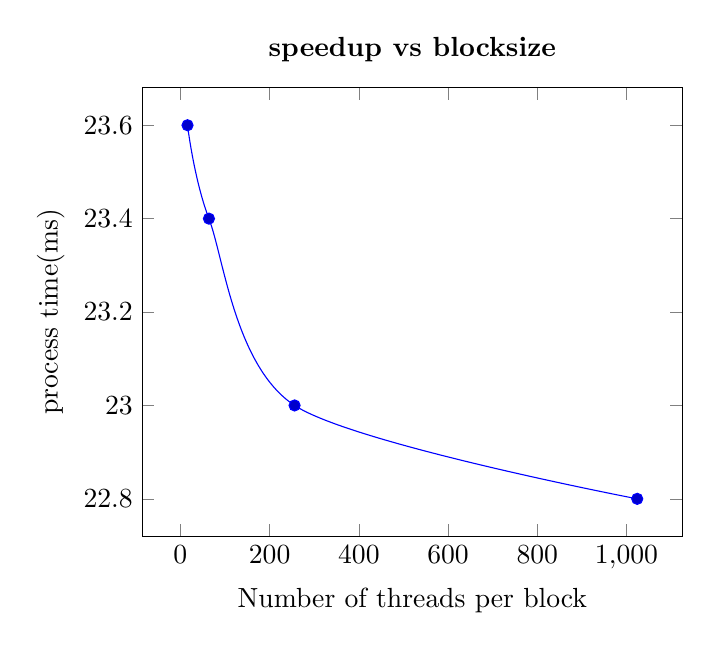
\begin{tikzpicture}
    \begin{axis}[title={\textbf{speedup vs blocksize}}, xlabel={Number of threads per     block}, ylabel={process time(ms)}]
        \addplot+[smooth,mark=*] plot coordinates
            {(16, 23.6) (64,23.4) (256,23.0) (1024, 22.8)};
    \end{axis}
\end{tikzpicture}
\newline
The process time increase with the number of threads per block as well. The process is also a bit slower than in 1D, but it's maybe because it did one more operation to compute TID.
\newline
\includegraphics[width=\textwidth]{labwork4-gpu-out.jpg}
\bibliographystyle{plain}
\end{document}
